%! Author = loreb
%! Date = 31/10/2023

\documentclass{article}

% Language setting
% Replace `english' with e.g. `spanish' to change the document language
\usepackage[italian]{babel}

% Set page size and margins
% Replace `letterpaper' with `a4paper' for UK/EU standard size
\usepackage[letterpaper,top=2cm,bottom=2cm,left=3cm,right=3cm,marginparwidth=1.75cm]{geometry}

% Useful packages
\usepackage{amsmath}
\usepackage{amsfonts}
\usepackage{graphicx}
\usepackage{mathrsfs}
\usepackage[colorlinks=true, allcolors=blue]{hyperref}
\usepackage{subcaption}
\usepackage{float}
\usepackage{wrapfig}

\usepackage[font=small,labelfont=bf]{caption}

\title{K-means and Mixed-Integer Quadratic Programming}
\author{Lorenzo Baiardi \& Thomas Del Moro}

\begin{document}
    \maketitle
    \begin{abstract}
        K-means è uno degli algoritmi più conosciuti e utilizzati per molti problemi di clustering. In questo lavoro analizziamo un approccio innovativo del k-means, basato sulla tecnica di Mixed-Integer Quadratic Programming (MIQP). Attraverso l'utilizzo di dataset sintetici e real-world valutiamo le performance di questo metodo, in modo da comprenderne le
        eventuali potenzialità e criticità in ambito empirico.
    \end{abstract}


    \section{Introduzione}

    Questo lavoro consiste nell'analisi sperimentale dell'approccio MIQP relativamente all'algoritmo K-Means. In particolare i nostri studi si concentrano su un confronto tra tale versione con quella originale, sulla base di vari aspetti quali la l'andamento della funzione obiettivo e il tempo di esecuzione al variare dei parametri del dataset utilizzato.

    \subsection{K-Means}

    Consideriamo un dataset numerico $D=\{x_i \in \mathbb{R}^{N}, i=1,\dots,n\}$. Applicare l'algoritmo K-Means significa partizionare gli esempi $x_i$ in $K$ cluster, con $K$ fissato, in modo da minimizzare la somma delle distanze euclidee al quadrato tra ogni elemento del dataset e il centroide del cluster al quale è assegnato.
    Formalmente il problema è dato da
    \begin{equation}
        \min_{\begin{subarray}{c}
                  \delta \in \{0, 1\}^{n \times K}\\
                  z \in \mathbb{R}^{K \times N}
        \end{subarray}}
        \frac{1}{2} \sum_{i=1}^{n} \sum_{k=1}^{K} \delta_{ik} \|x_i-z_k\|^2
        \label{eq:kmeans}
    \end{equation}
    dove $\delta_{ik}$ sono le variabili indicatrici dell'associazione tra l'esempio $x_i$ e il cluster $k$, mentre le $z_k$ indentificano il centroide del cluster $k$.\\
    A questo problema sono poi stati aggiunti dei vincoli in modo da ottenere un problema di Hard Clustering bilanciato, per cui ogni punto può essere associato a un solo cluster e ad ogni cluster devono essere associati almeno $C$ elementi. Dunque il problema diventa
    \begin{equation}
        \begin{aligned}
            \min_{\substack{
                \delta \in \{0, 1\}^{n \times K}\\
                z \in \mathbb{R}^{K \times N}}} &
            \frac{1}{2} \sum_{i=1}^{n} \sum_{k=1}^{K} \delta_{ik} \|x_i-z_k\|^2 \\
            \text{t.c.} \quad &
            \begin{aligned}
                & \sum_{k=1}^{K} \delta_{ik} = 1 \quad \text{for $i=1,\dots,n$}\\
                & \sum_{i=1}^{n} \delta_{ik} \geq C_k \quad \text{for $k=1,\dots,K$}
            \end{aligned}
        \end{aligned}
        \label{eq:constrained_kmeans}
    \end{equation}

    In questa formulazione l'algoritmo viene inizializzato con dei centroidi casuali, dopodiché ripete iterativamente i seguenti due step:
    \begin{itemize}
        \item \textbf{Assegnazione}: ogni elemento $x_i$ viene assegnato al cluster $k$ il cui centroide è più vicino a $x_i$ tra tutti i centroidi
        \[\delta^{t+1} \in \arg \min_{\delta \in \{0,1\}^n\times \K} \frac{1}{2} \sum_{i=1}^{n} \sum_{k=1}^{K} \delta_{ik} \|x_i-z_k^{t}\|^2\]
        \item \textbf{Aggiornamento}: tutti i centroidi vengono aggiornati come la media dei punti assegnati al loro cluster
        \[z^{t+1} \in \arg \min_{z} \frac{1}{2} \sum_{i=1}^{n} \sum_{k=1}^{K} \delta_{ik}^{t+1} \|x_i-z_k\|^2\]
        in particolare si può verificare che vale la soluzione calcolabile in forma chiusa
        \[z_k^{t+1} = \frac{\sum_{i=1}^{n} \delta_{ik}^{t+1} x_i}{\sum_{i=1}^{n} \delta_{ik}^{t+1}}\]
    \end{itemize}

    \subsection{MIQP K-Means}
    Il MIQP (acronimo di Mixed-Integer Quadratic Programming) è una combinazione di Quadratic Programming e Mixed-Integer Linear Programming, più in particolare è una classe di problemi di ottimizzazione che consiste nel minimizzare una funzione quadratica di variabili continue soggette a vincoli lineari, ma alcune delle variabili sono anche soggette a vincoli di interezza.\\
    Molti problemi di ottimizzazione possono essere riformulati come MIQP e risolti attraverso l'utilizzo di solver (es. Gurobi) che oggi sono capaci di gestire un gran numero di variabili intere e trovare l'ottimo globale del problema.\\
    Nel nostro caso, quindi, il problema di clustering può essere riformulato in modo da garantire, tramite l'utilizzo di un solver, il raggiungimento dell'ottimo globale; in contrasto con la versione classica di K-Means che è soggetta allo stazionamento in minimi locali.\\
    Il problema~\ref{eq:constrained_kmeans} può dunque essere riformulato come
    \begin{equation}
        \begin{aligned}
            \min_{\substack{
                \delta \in \{0, 1\}^{n \times K}\\
                z \in \mathbb{R}^{K \times N} \\
                s \in \mathbb{R}^{N \times n \times K}}} &
            \frac{1}{2} \sum_{i=1}^{n} \sum_{k=1}^{K} \|s_{ik}\|^2 \\
            \text{t.c.} \quad &
            \begin{aligned}
                & \sum_{k=1}^{K} \delta_{ik} = 1 \quad \text{for $i=1,\dots,n$} \\
                & \sum_{i=1}^{n} \delta_{ik} \geq C_k \quad \text{for $k=1,\dots,K$} \\
                & -M(1-\delta_{ik}) + (x_{ij}-z_{kj}) \leq s_{jik} \leq M(1-\delta_{ik}) + (x_{ij}-z_{kj}) \quad \text{for all $i, j, k$}
            \end{aligned}
        \end{aligned}
        \label{eq:MIQkmeans}
    \end{equation}
    dove $M$ è un valore sufficientemente grande da garantire che:
    \begin{itemize}
        \item se $\delta_{ik} = 0$ allora $s_{jik}$ sia uguale alla distanza tra $x_{ij}$ e $z_{kj}$.
        \item se $\delta_{ik} = 1$ allora $s_{jik}$ sia libero e quindi settato a 0.
    \end{itemize}

    \section{Implementazione}
    Il software è stato realizzato in linguaggio Python, utilizzando il solver Gurobi per la risoluzione dei problemi di ottimizzazione. Sono state implementate due classi, rispettivamente per la versione vanilla di K-Means e per la versione MIQP. Nel codice sono poi presenti funzioni per la generazione di dataset artificiali e per la realizzazione dei grafici.\\
    L'algoritmo K-Means viene inizializzato con un numero fissato di centroidi presi casualmente tra i punti del dataset. Gli indicatori (variabili di associazione tra dato e cluster) sono considerati come unica variabile del problema; vengono assegnati iterativamente attraverso l'ottimizzazione del solver Gurobi e memorizzati in un dizionario Python. Per l'aggiornamento dei centroidi, invece, viene utilizzato il calcolo in forma chiusa mostrato sopra.\\
    La versione MIQP invece si basa interamente sull'ottimizzazione del solver Gurobi. In questo caso, oltre agli indicatori, diventano variabili anche i centroidi e i residui, che verranno utilizzati per il calcolo della funzione obiettivo. Il valore della costante $M$ utilizzata nei vincoli è stata approssimata a un valore sufficientemente grande da non introdurre vincoli di box, ma allo stesso tempo abbastanza piccolo in modo da migliorare l'efficienza dell'algoritmo.\\

    \section{Esperimenti e Risultati}
    Entrambi gli algoritmi sono stati testati su dataset sintetici e real-world osservando principalmente il valore della funzione obiettivo e il tempo di esecuzione. In particolare sono stati confrontati tali risultati al variare dei fattori $n$, $N$, e $K$, in modo da comprendere le eventuali criticità delle due formulazioni del problema. Tutti gli esperimenti sono stati eseguiti su un processore Intel Core i7-8565U con 8GB di ram, utlizzando il software Gurobi 10.0.2\\
    \subsection{Test visuali}
    Prima di tutto sono stati eseguiti alcuni test visuali per analizzare il comportamento dei due algoritmi. Per farlo, è stato utilizzato un algoritmo di PCA, che ha permesso di costruire uno scatterplot in due dimensioni dei dati clusterizzati. In Figura \ref{fig:scatter_cluster} sono mostrati alcuni esempi di clustering ottenuti con la versione MIQP di K-Means eseguito su dataset di 1000 elementi e 3 features generati artificialmente con distribuzione uniforme.
    \begin{figure}[h]
     \centering
     \begin{subfigure}[b]{0.32\linewidth}
         \centering
         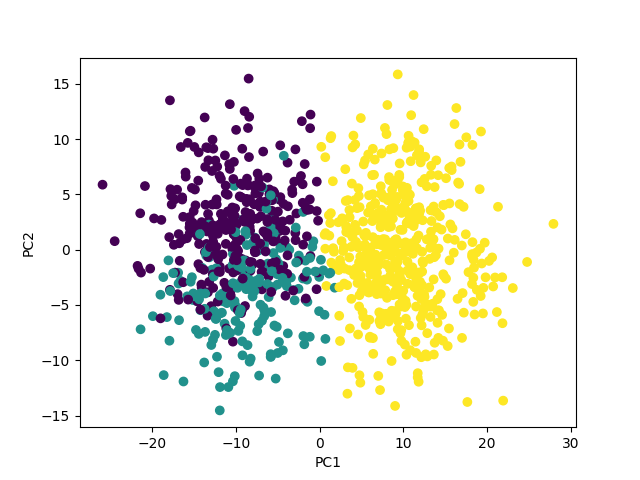
\includegraphics[width=\linewidth]{../results/plots/scatter_k3}
         \caption{3 cluster}
     \end{subfigure}
     \hfill
     \begin{subfigure}[b]{0.32\linewidth}
         \centering
         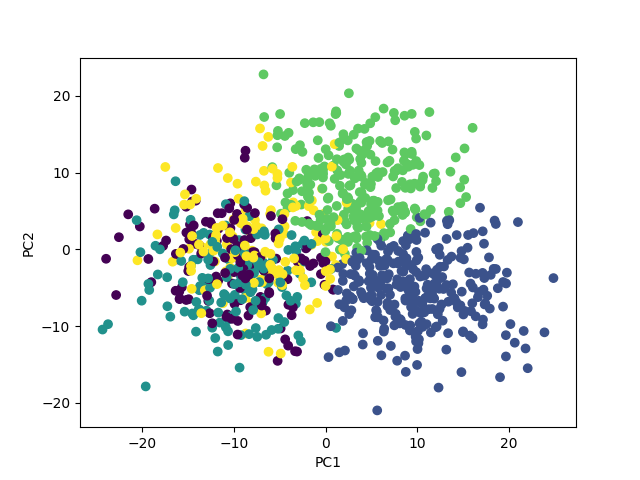
\includegraphics[width=\linewidth]{../results/plots/scatter_k5}
         \caption{5 cluster}
     \end{subfigure}
     \begin{subfigure}[b]{0.32\linewidth}
         \centering
         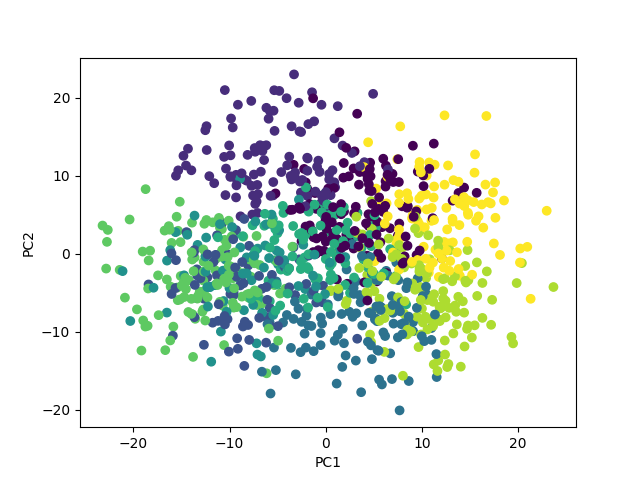
\includegraphics[width=\linewidth]{../results/plots/scatter_k7}
         \caption{7 cluster}
     \end{subfigure}
     \caption{Scatterplot dei dati clusterizzati con MIQP K-Means}
     \label{fig:scatter_cluster}
    \end{figure}
    In tutti i casi è stato impostato un time-limit per la versione MIQP per ottenere i risultati in tempi ragionevoli. Ciò ovviamente porta a ottenere una soluzione sub-ottima anche con questa versione del'algoritmo. Tuttavia, poiché il funzionamento degli algoritmi è diverso, anche tale soluzione sub-ottima sarà probabilmente diversa. In Figura \ref{fig:scatter_version} sono stati riportati i cluster ottenuti con i due algoritmi su un dataset artificiale di 1000 elementi e 2 features. Come è possibile notare in figura K-Means costruisce sempre cluster di forma globulare; diversamente, la versione MIQP (con time-limit) può essere interrotta prima di aver assegnato ogni punto al cluster più vicino. Sarà più probabile, quindi, avere dei cluster più omogenei in cui però alcuni punti singolari potranno essere etichettati in modo evidentemente errato.
    \begin{figure}[h]
     \centering
     \begin{subfigure}[b]{0.49\linewidth}
         \centering
         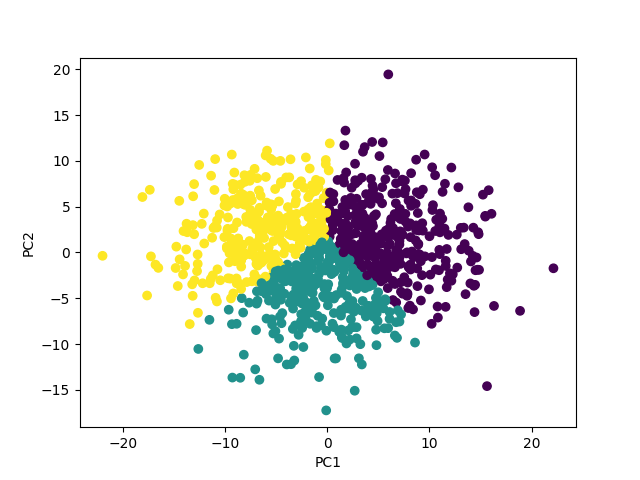
\includegraphics[width=\linewidth]{../results/plots/scatter_carino_kmeans}
         \caption{K-Means}
     \end{subfigure}
     \begin{subfigure}[b]{0.49\linewidth}
         \centering
         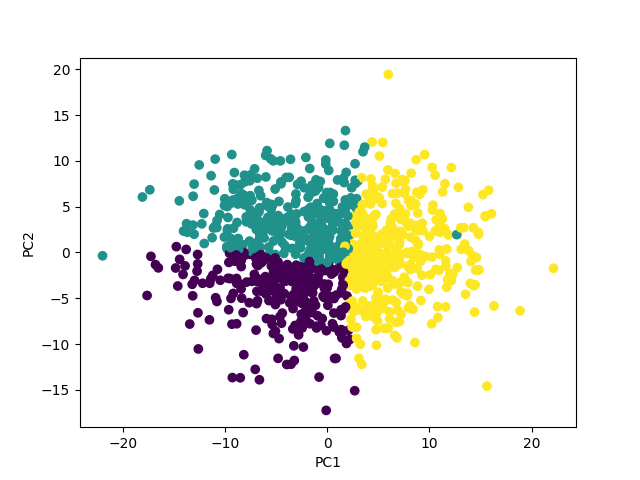
\includegraphics[width=\linewidth]{../results/plots/scatter_carino}
         \caption{MIQP K-Means}
     \end{subfigure}
     \caption{Scatterplot dei dati clusterizzati}
     \label{fig:scatter_version}
    \end{figure}

\clearpage

    \subsection{Dataset sintetici}
    \begin{wrapfigure}{R}{0.40\textwidth}
    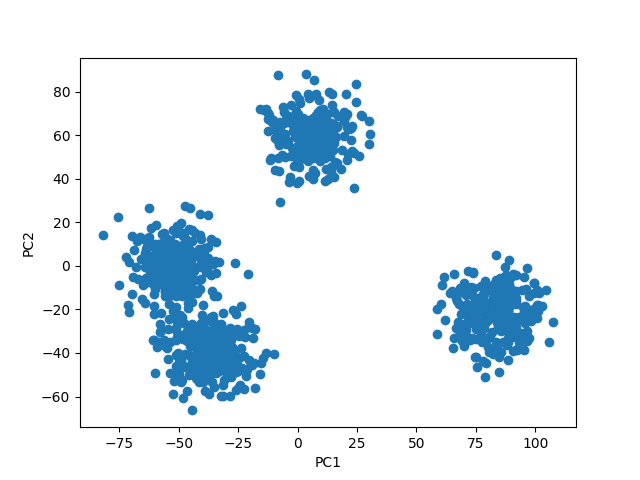
\includegraphics[width=1\linewidth]{../results/plots/dataset1}
    \caption{Scatterplot del primo dataset sintetico}
    \label{sint}
    \end{wrapfigure}

    Gli algoritmi sono poi stati confrontati anche in termini di risultati quantitativi, prima su dati sintetici manipolabili, poi su dataset real-world.
    Il primo dataset preso in considerazione è stato generato in modo da essere costituito da più cluster facilmente distinguibili. Si tratta di un dataset di 1000 elementi con 10 features ciascuno, generati da 4 diversi centroidi. In Figura \ref{sint} è mostrato uno scatterplot delle prime due componenti principali di tale dataset.

    Gli esperimenti sono stati eseguiti su sottoinsiemi di tale dataset, specificamente al variare di tre parametri fondamentali, ovvero il numero di esempi nel dataset, il numero di feature di tali elementi e il numero di cluster in cui raggruppare i dati. In tutti i casi è stato impostato un time-limit di 1000 secondi per la versione MIQP, in modo da ottenere risultati significativi in tempi ragionevoli.\\
    Per prima cosa, sono stati fissati il numero di cluster $K=3$ e il numero di feature $N=4$, mentre il numero di elementi è stato fatto variare in $n=10,20,\dots,80$. Ad ogni iterazione viene eseguito un mescolamento dei dati, in modo da prendere sempre elementi diversi. In Figura~\ref{fig:size_sint} sono mostrati i risultati ottenuti. Attraverso un'analisi real-time è stato possibile riportare (in rosso) il tempo necessario alla versione MIQP per raggiungere una soluzione migliore del competitor, ovviamente quando questa è stata raggiunta in periodi inferiori al time-limit impostato.
    Risulta evidente che all'aumentare del numero di esempi nel dataset, la versione MIQP impiega sempre più tempo per raggiungere la soluzione ottima. In particolare, per dataset di dimensioni maggiori di 50 elementi, la versione MIQP non riesce a raggiungere la soluzione sub-ottima ottenuta con K-means in tempi ragionevoli. Si può notare che anche K-Means sia influenzato dal numero di esempi, tuttavia in modo molto meno significativo.\\
    \begin{figure}[H]
     \centering
     \begin{subfigure}[t]{0.49\linewidth}
         \centering
         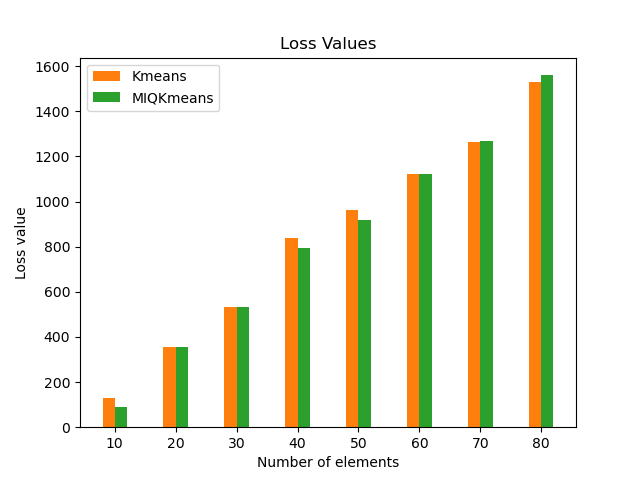
\includegraphics[width=\linewidth]{../results/log_plots/loss_size_sint}
         \caption{Valore finale della funzione obiettivo}
     \end{subfigure}
     \hfill
     \begin{subfigure}[t]{0.49\linewidth}
         \centering
         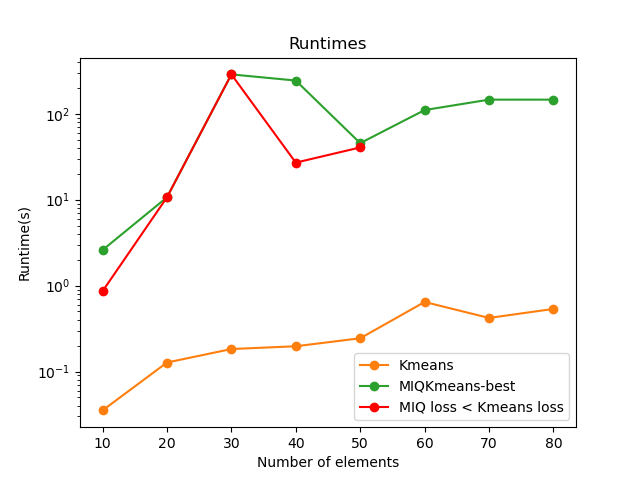
\includegraphics[width=\linewidth]{../results/log_plots/runtime_size_sint_log}
         \caption{Tempo di esecuzione: tempo impiegato da Kmeans per raggiungere la soluzione sub-ottimale (arancio); tempo impiegato da MIQP per raggiungere la migliore soluzione trovata (verde); tempo impiegato da MIQP per raggiungere una soluzione migliore di Kmeans (rosso)}
     \end{subfigure}
        \caption{Performance al variare del numero di elementi}
        \label{fig:size_sint}
     \end{figure}
    Allo stesso modo è aspettabile che anche il numero di cluster scelto possa influenzare le performance dell'algoritmo. In Figura \ref{fig:k_sint} sono mostrati i risultati ottenuti fissando il numero di elementi $n=40$ e il numero di feature $N=4$. In particolare il numero di centroidi con cui viene inizializzato l'algoritmo sembra essere un fattore ancora più significativo per le performance della versione MIQP.
    Mentre l'algoritmo Kmeans sembra non subire grandi variazioni dovute all'aumento del numero di cluster, quest'ultimo ragionevolemnte implica un importante crescita del numero di variabili binarie che devono essere gestite dal solver per la versione MIQP.\\
    \begin{figure}[H]
     \centering
     \begin{subfigure}[t]{0.49\linewidth}
         \centering
         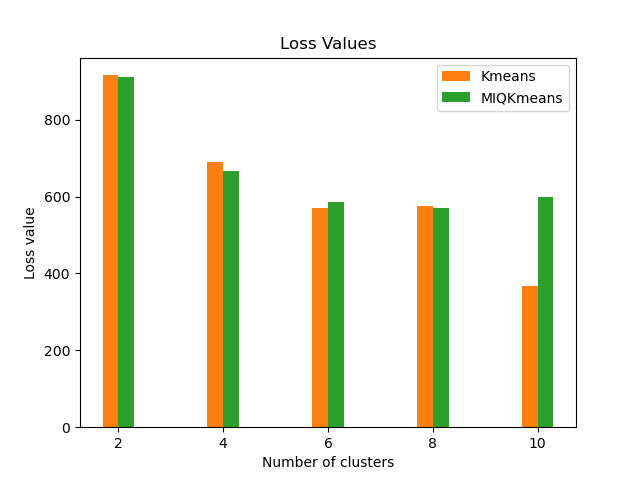
\includegraphics[width=\linewidth]{../results/log_plots/loss_centers_sint}
         \caption{Valore finale della funzione obiettivo}
     \end{subfigure}
     \hfill
     \begin{subfigure}[t]{0.49\linewidth}
         \centering
         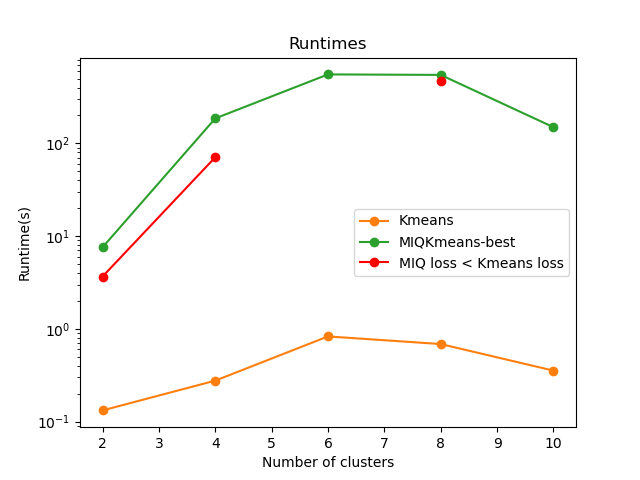
\includegraphics[width=\linewidth]{../results/log_plots/runtime_centers_sint_log}
         \caption{Tempo di esecuzione: tempo impiegato da Kmeans per raggiungere la soluzione sub-ottimale (arancio); tempo impiegato da MIQP per raggiungere la migliore soluzione trovata (verde); tempo impiegato da MIQP per raggiungere una soluzione migliore di Kmeans (rosso)}
     \end{subfigure}
        \caption{Performance al variare del numero di cluster}
        \label{fig:k_sint}
     \end{figure}
    Diversamente, il numero di feature non varia la quantità di variabili di associazione tra esempi e cluster, dunque dovrebbe avere un'influenza minore sulla differenza di performance tra i due algoritmi. Si può infatti osservare in Figura \ref{fig:f_sint} che con quasi tutti i valori di $N$ testati, sempre fissando $n=40$ e $K=3$ la variante MIQP riesce a raggiungere la soluzione sub-ottima ottenuta con K-means in tempi ragionevoli. È comunque presente una netta correlazione tra il numero di feature e il tempo di esecuzione della versione MIQP. Tale correlazione non sembra invece presente in K-Means.\\
    \begin{figure}[H]
     \centering
     \begin{subfigure}[t]{0.49\linewidth}
         \centering
         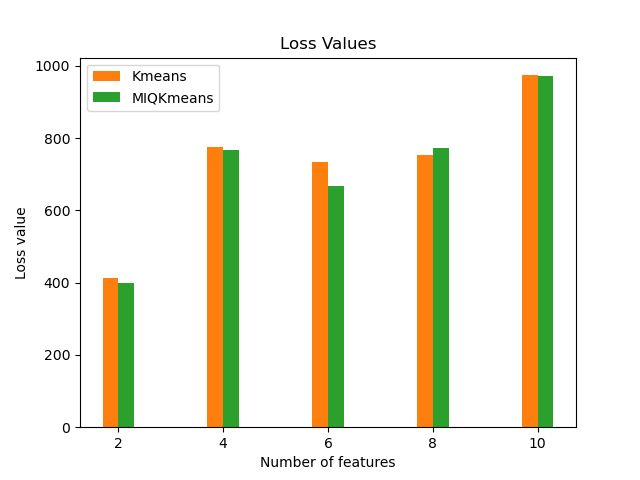
\includegraphics[width=\linewidth]{../results/log_plots/loss_features_sint}
         \caption{Valore finale della funzione obiettivo}
     \end{subfigure}
     \hfill
     \begin{subfigure}[t]{0.49\linewidth}
         \centering
         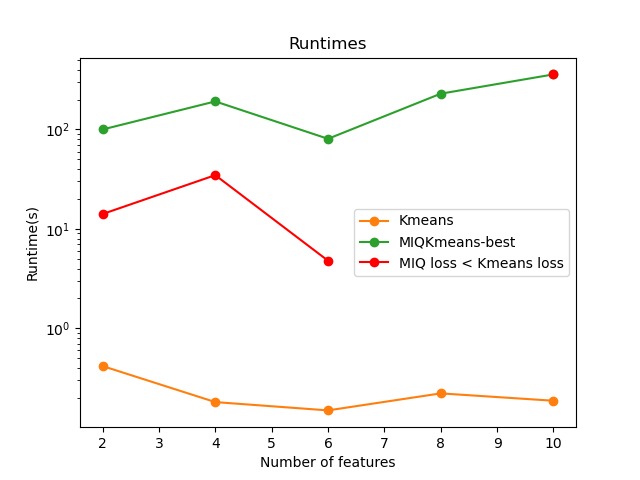
\includegraphics[width=\linewidth]{../results/log_plots/runtime_features_sint_log}
         \caption{Tempo di esecuzione: tempo impiegato da Kmeans per raggiungere la soluzione sub-ottimale (arancio); tempo impiegato da MIQP per raggiungere la migliore soluzione trovata (verde); tempo impiegato da MIQP per raggiungere una soluzione migliore di Kmeans (rosso)}
     \end{subfigure}
        \caption{Performance al variare del numero di features}
        \label{fig:f_sint}
     \end{figure}
    Dai test effettuati fin qui si può dedurre che in tutti i casi il tempo di esecuzione della versione MIQP dell'algoritmo è di gran lunga maggiore. D'altra parte, se si lavora con un insieme di dati relativamente piccolo, si riescono a ottenere cluster migliori anche in tempi ragionevoli.\\
    Come era prevedibile la formulazione MIQP è particolarmente sensibile al numero di variabili binarie del problema \cite{lapucci}. Sia variando la dimensione del dataset che il numero di cluster è possibile notare che un numero di variabili intere superiore al valore approssimativo di 150 porta in quasi tutti i casi a un tempi dell'ordine delle migliaia di secondi per raggiungere la soluzione sub-ottima ottenuta con K-Means.\\

    \begin{wrapfigure}{R}{0.40\textwidth}
    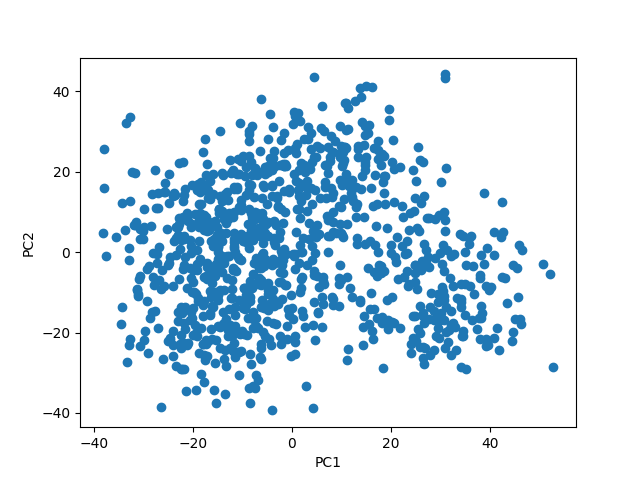
\includegraphics[width=1\linewidth]{../results/plots/dataset2}
    \caption{Scatterplot del secondo dataset sintetico}
    \label{sint_sint}
    \end{wrapfigure}
    Dopodiché sono stati replicati gli stessi esperimenti su un dataset con cluster molto meno distinguibili. Si tratta di un dataset di 1000 esempi con 10 features, generati a partire da 5 cluster diversi ma con poca distanza tra i centroidi. Lo scatterplot delle due componenti principali è riportato in Figura \ref{sint_sint}.\\
    I risultati ottenuti sono molto simili ai precedenti, tuttavia è possibile notare che la versione MIQP riesce a superare la soluzione sub-ottima ottenuta con K-means anche per dataset di dimensioni maggiori (in questo caso il numero di elementi è stato variato nell'intervallo $n=20,\dots,120$). Ciò potrebbe dipendere dal fatto che K-Means fosse avvantaggiato dalla lontananza tra i diversi cluster generati.\\
    In questo caso risulta più evidente che del numero di features abbia un impatto molto minore sul tempo di esecuzione della formulazione MIQP.\\
    \begin{figure}[h]
     \begin{subfigure}{0.32\linewidth}
         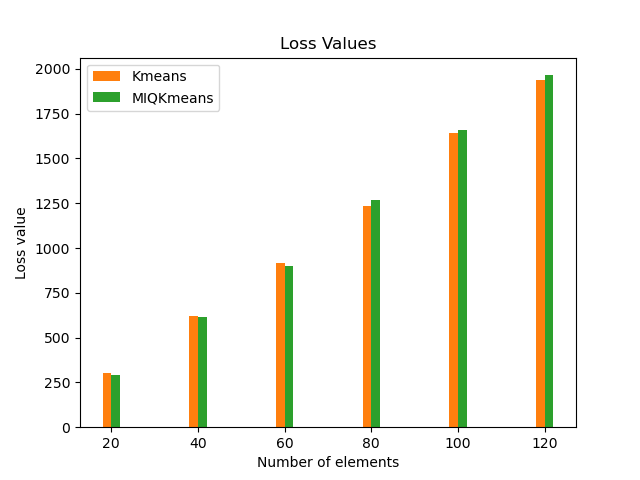
\includegraphics[width=\linewidth]{../results/log_plots/loss_size_sint2}
     \end{subfigure}%
     \begin{subfigure}{0.32\linewidth}
         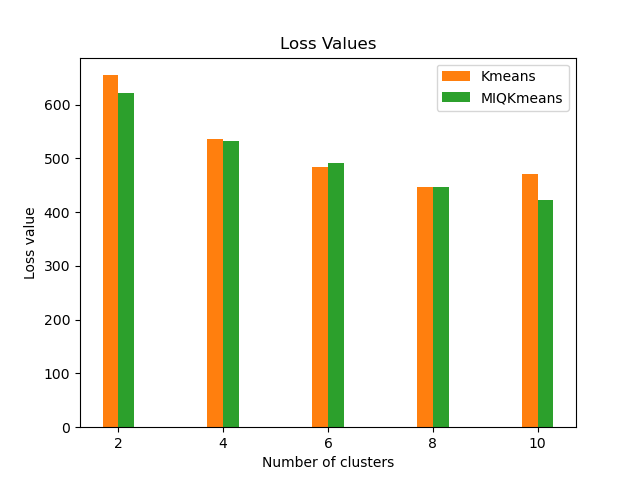
\includegraphics[width=\linewidth]{../results/log_plots/loss_centers_sint2}
     \end{subfigure}%
     \begin{subfigure}{0.32\linewidth}
         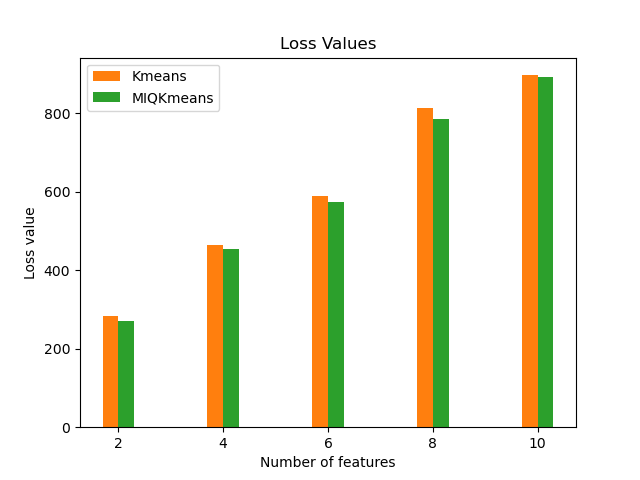
\includegraphics[width=\linewidth]{../results/log_plots/loss_features_sint2}
     \end{subfigure}
     \begin{subfigure}{0.32\linewidth}
         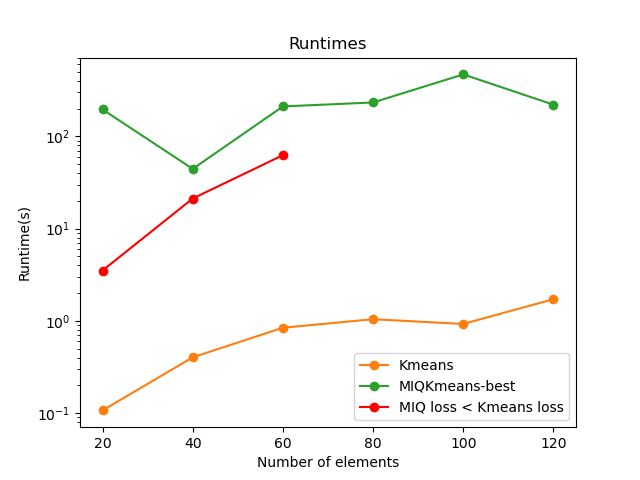
\includegraphics[width=\linewidth]{../results/log_plots/runtime_size_sint2_log}
     \end{subfigure}%
     \begin{subfigure}{0.32\linewidth}
         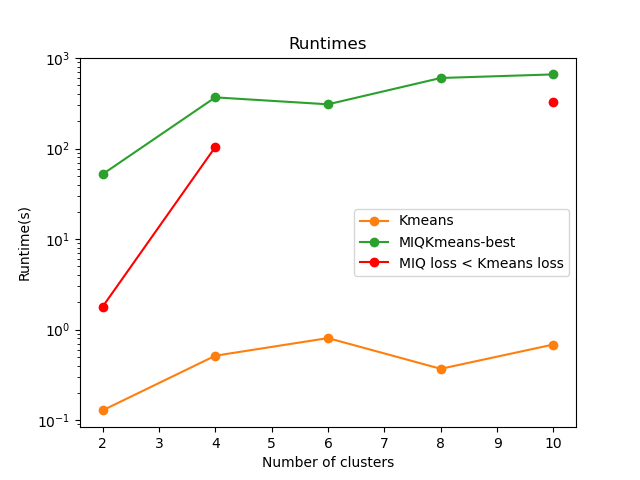
\includegraphics[width=\linewidth]{../results/log_plots/runtime_centers_sint2_log}
     \end{subfigure}%
     \begin{subfigure}{0.32\linewidth}
         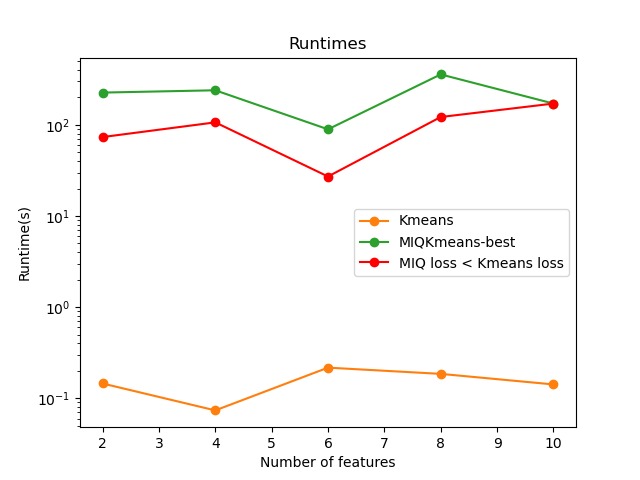
\includegraphics[width=\linewidth]{../results/log_plots/runtime_features_sint2_log}
     \end{subfigure}%
     \caption{Performance al variare del numero di elementi, cluster e features}
     \label{fig:runtime_loss_sint2}
    \end{figure}

    \subsection{Dataset real-world}
    In questa sezione analizziamo gli esperimenti svolti su un dataset real-world. Il dataset considerato è Heart Disease Patients. Contiene 303 esempi di 11 feature di varie tipologie.
    Gli esperimenti sono stati eseguiti su sottoinsiemi di tale dataset con caratteristiche diverse. Anche in questo caso, infatti, sono stati variati parametri quali numero di esempi, numero di features e numero di cluster. In tutti i casi è stato impostato un time-limit per la versione MIQP, in modo da ottenere risultati significativi in tempi ragionevoli.\\
    La Figura \ref{fig:size_real} mostra i risultati ottenuti al variare del numero di elementi del dataset, fissando il numero di features $N=4$ e il numero di cluster $K=3$. Come già accennato in precedenza, la versione MIQP dovrebbe essere particolarmente sensibile al numero di variabili binarie del problema; poiché il numero di elementi è fatto variare in $n=20,\dots,120$, il numero di variabili in gioco ha un un minimo di 60 e un massimo di 360.\\
    \begin{figure}[H]
     \centering
     \begin{subfigure}[t]{0.49\linewidth}
         \centering
         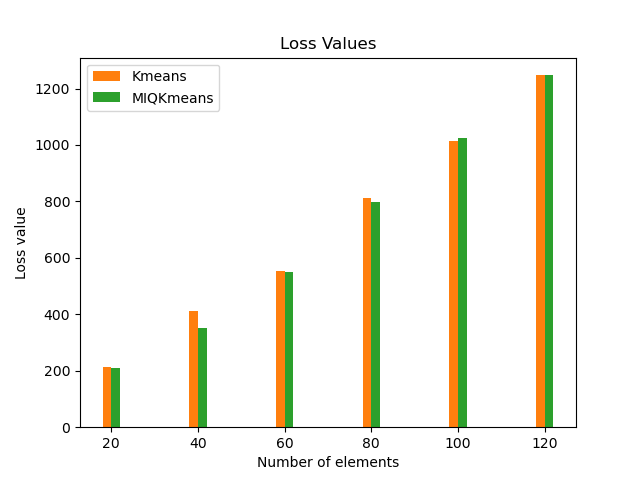
\includegraphics[width=\linewidth]{../results/log_plots/loss_size_heart}
         \caption{Valore finale della funzione obiettivo}
     \end{subfigure}
     \hfill
     \begin{subfigure}[t]{0.48\linewidth}
         \centering
         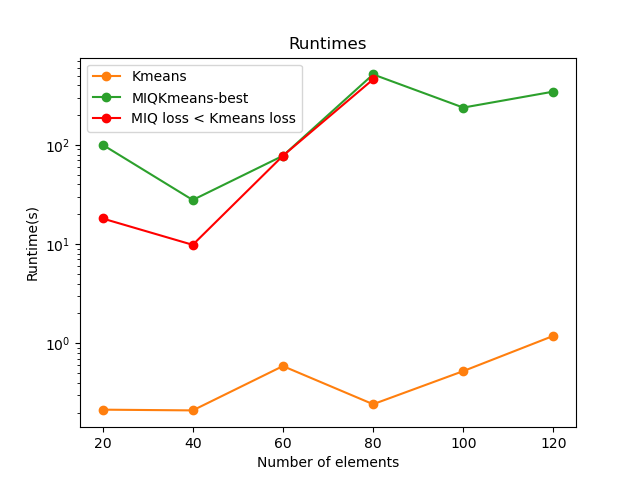
\includegraphics[width=\linewidth]{../results/log_plots/runtime_size_heart_log}
         \caption{Tempo di esecuzione: tempo impiegato da Kmeans per raggiungere la soluzione sub-ottimale (arancio); tempo impiegato da MIQP per raggiungere la migliore soluzione trovata (verde); tempo impiegato da MIQP per raggiungere una soluzione migliore di Kmeans (rosso)}
     \end{subfigure}
        \caption{Performance al variare del numero di elementi}
        \label{fig:size_real}
     \end{figure}
    Risulta evidente che all'aumentare del numero di esempi nel dataset, la versione MIQP impiega sempre più tempo per raggiungere la soluzione ottima. Nonostante ciò sembra che in questo caso la quantità di variabili gestibili dal solver possa essere maggiore, in quanto l'algoritmo è riuscito a fare meglio di K-Means in tempi inferiori al time-limit di 1000 secondi anche per dataset più grandi.\\
    Allo stesso modo è aspettabile che anche il numero di cluster scelto possa influenzare le performance dell'algoritmo. In Figura \ref{fig:k_real} sono mostrati i risultati ottenuti fissando il numero di elementi $n=40$ e il numero di features $N=4$. Anche per quanto riguarda il numero di cluster, sembra che la versione MIQP possa essere in grado di gestire un numero maggiore di variabili rispetto ai casi precedenti.
    \begin{figure}[H]
     \centering
     \begin{subfigure}[t]{0.485\linewidth}
         \centering
         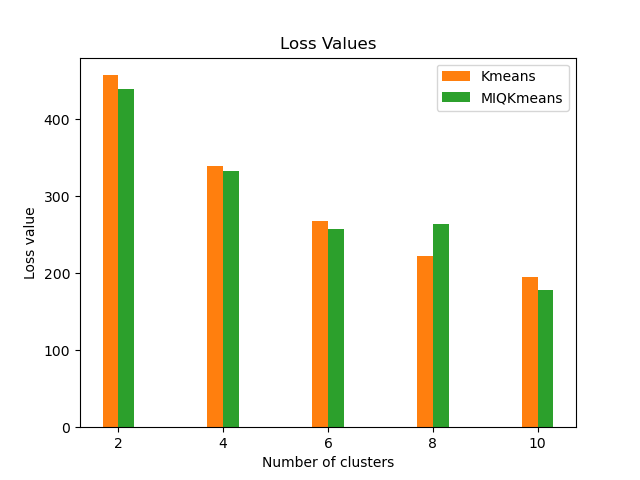
\includegraphics[width=\linewidth]{../results/log_plots/loss_centers_heart}
         \caption{Valore finale della funzione obiettivo}
     \end{subfigure}
     \hfill
     \begin{subfigure}[t]{0.49\linewidth}
         \centering
         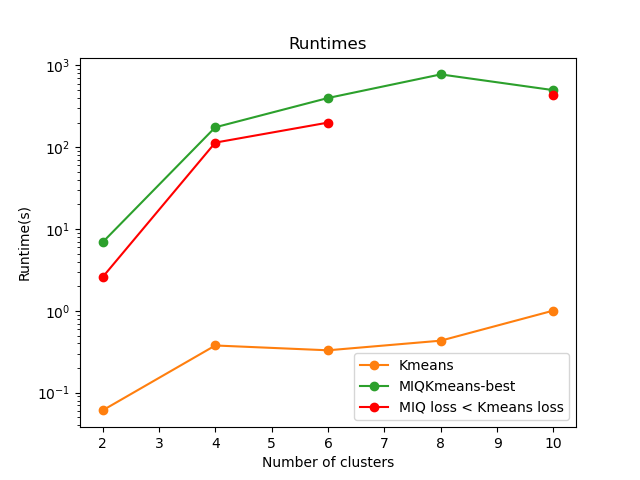
\includegraphics[width=\linewidth]{../results/log_plots/runtime_centers_heart_log}
         \caption{Tempo di esecuzione: tempo impiegato da Kmeans per raggiungere la soluzione sub-ottimale (arancio); tempo impiegato da MIQP per raggiungere la migliore soluzione trovata (verde); tempo impiegato da MIQP per raggiungere una soluzione migliore di Kmeans (rosso)}
     \end{subfigure}
        \caption{Performance al variare del numero di cluster}
        \label{fig:k_real}
     \end{figure}
    Diversamente, il numero di feature non varia la quantità di variabili di associazione tra esempi e cluster, dunque dovrebbe avere un'influenza minore sulla differenza di performance. Si può infatti osservare in Figura \ref{fig:f_real} che con tutti i valori di $N$ testati, sempre fissando $n=40$ e $K=3$, la variante MIQP riesce a raggiungere la soluzione sub-ottima ottenuta con K-means in tempi ragionevoli.
    \begin{figure}[H]
     \centering
     \begin{subfigure}[t]{0.49\linewidth}
         \centering
         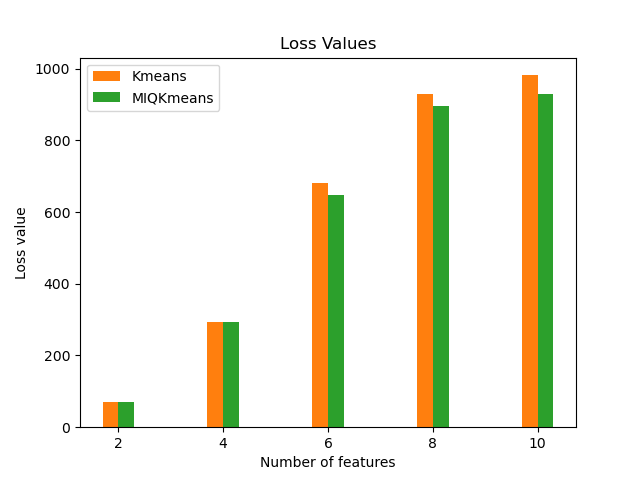
\includegraphics[width=\linewidth]{../results/log_plots/loss_features_heart}
         \caption{Valore finale della funzione obiettivo}
     \end{subfigure}
     \hfill
     \begin{subfigure}[t]{0.49\linewidth}
         \centering
         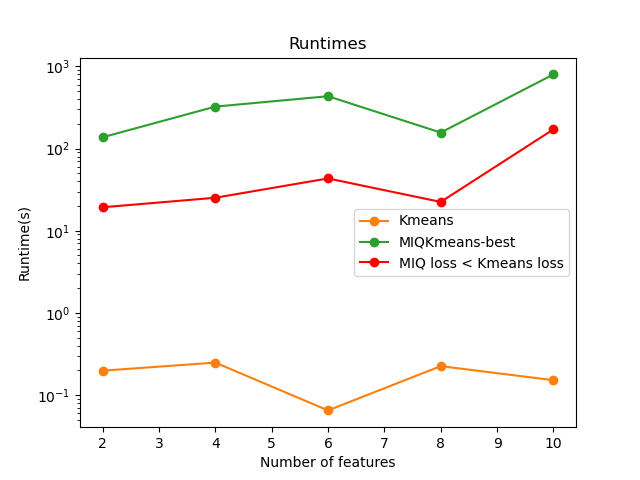
\includegraphics[width=\linewidth]{../results/log_plots/runtime_features_heart_log}
         \caption{Tempo di esecuzione: tempo impiegato da Kmeans per raggiungere la soluzione sub-ottimale (arancio); tempo impiegato da MIQP per raggiungere la migliore soluzione trovata (verde); tempo impiegato da MIQP per raggiungere una soluzione migliore di Kmeans (rosso)}
     \end{subfigure}
        \caption{Performance al variare del numero di features}
        \label{fig:f_real}
     \end{figure}
    I risultati ottenuti con il dataset Heart Disease Patients sono molto simili a quelli ottenuti con i dataset sintetici. In particolare, anche in questo caso la versione MIQP è particolarmente sensibile al numero di variabili binarie del problema, ma sembra che riesca a ottenere buoni risultati anche fino alle 240 variabili.

    \subsection{Inizializzazioni multiple di K-Means}
    Infine, è stato eseguito un ulteriore esperimento per valutare le performance della versione MIQP rispetto a K-Means. In particolare, ad ogni iterazione è stato eseguito K-Means più volte, inizializzando ogni volta i centroidi con un set di punti diverso, per poi scegliere la soluzione migliore trovata tra tutte le esecuzioni. In questo modo è stato possibile ottenere una soluzione sub-ottima migliore rispetto a quella ottenuta con una singola esecuzione dell'algoritmo.
    Il test è stato effettuato di nuovo sul dataset Heart Disease Patients, fissando il numero di feature $N=4$ e variando il numero di variabili binarie nel range $120,...,300$. Il numero di diverse esecuzioni di K-Means è stato fissato a 10.\\
    \begin{figure}[h]
        \centering
        \begin{subfigure}[t]{0.49\linewidth}
            \centering
            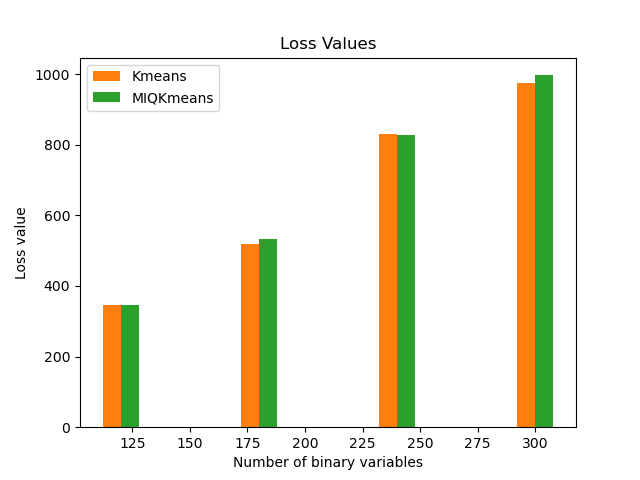
\includegraphics[width=\linewidth]{../results/log_plots/loss_multiple_inits_heart}
            \caption{Valore finale della funzione obiettivo}
        \end{subfigure}
        \hfill
        \begin{subfigure}[t]{0.49\linewidth}
            \centering
            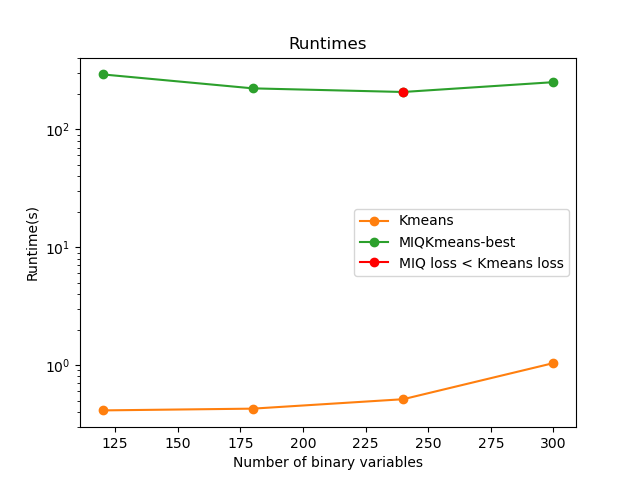
\includegraphics[width=\linewidth]{../results/log_plots/runtime_multiple_inits_heart_log}
            \caption{Tempo di esecuzione: tempo impiegato da tutte le esecuzioni di Kmeans per raggiungere la soluzione sub-ottimale (arancio); tempo impiegato da MIQP per raggiungere la migliore soluzione trovata (verde); tempo impiegato da MIQP per raggiungere una soluzione migliore di Kmeans (rosso)}
        \end{subfigure}
            \caption{Performance al variare del numero di variabili binarie del problema}
            \label{fig:multi_init}
    \end{figure}
    In Figura \ref{fig:multi_init} sono riportati i risultati ottenuti, in particolare per K-Means i tempi sono da considerarsi complessivi di tutte le esecuzioni. Come è possibile osservare nel caso in cui l'algoritmo K-Means venga eseguito più volte a partire da diversi centroidi iniziali, la migliore soluzione ottenuta è difficilmente raggiungibile dalla versione MIQP in tempi brevi. Si deve inoltre notare che, nonostante K-Means sia eseguito 10 volte, il tempo totale impiegato per l'esecuzione rimane di gran lunga inferiore rispetto alla singola iterazione dell'algoritmo MIQP.

    \section{Conclusioni}
    In questo lavoro è stato analizzato un approccio innovativo di K-Means, basato sulla tecnica di Mixed-Integer Quadratic Programming (MIQP). Attraverso l'utilizzo di dataset sintetici e real-world sono state valutate le performance di questo metodo, in modo da valutarne vantaggi e svantaggi in ambito empirico.\\
    Dai risultati ottenuti è possibile dedurre che la versione MIQP dell'algoritmo K-Means è particolarmente sensibile al numero di variabili binarie del problema, al cui aumento corrisponde una sempre peggiore efficienza. Ciò si verifica già con dataset dell'ordine delle decine di elementi, specialmente se devono essere raggruppati in un discreto numero di cluster.
    Inoltre abbiamo notato che eseguendo più volte K-Means si ottengono in poco tempo valori di loss minori, per raggiungere i quali la versione MIQP ha bisogno di tempi relativamente lunghi.
    Si può dunque supporre che l'approccio MIQP garantisca teoricamente il raggiungimento dell'ottimo globale, ma non sia facilmente scalabile in ambito pratico sulla quantità di dati processabili al giorno d'oggi.


    \begin{thebibliography}{9}
\bibitem{lapucci}
Matteo Lapucci, Davide Pucci (2023) \emph{Mixed-integer quadratic programming reformulations of multi-task learning models}

\bibitem{c-kmeans}
P. S. Bradley, K. P. Bennett, A. Demiriz (2000) \emph{Constrained K-Means Clustering}

\bibitem{b-kmeans}
Mikko I. Malinen, Pasi Fränti (2014) \emph{Balanced K-Means for Clustering}

\end{thebibliography}

\end{document}
